\documentclass{beamer}
\usepackage[utf8]{inputenc}

\usetheme{Madrid}
\usecolortheme{default}
\useinnertheme{circles}

\definecolor{Logo1}{rgb}{0.208, 0.2865, 0.373}
\definecolor{Logo2}{rgb}{0.000, 0.674, 0.863}

\setbeamercolor*{palette primary}{bg=Logo1, fg=white}
\setbeamercolor*{palette secondary}{bg=Logo2, fg=white}
\setbeamercolor*{palette tertiary}{bg=white, fg=Logo1}
\setbeamercolor*{palette quaternary}{bg=Logo1,fg=white}
\setbeamercolor{structure}{fg=Logo1} % itemize, enumerate, etc
\setbeamercolor{section in toc}{fg=Logo1} % TOC sections

\usepackage{graphicx,animate}
%------------------------------------------------------------
%This block of code defines the information to appear in the
%Title page
\title[Linear Algebra] %optional
{Basis \& Dimension; The Four Fundamental Subspaces}

\subtitle{Lecture 4}

\author[11910803@mail.sustech.edu.cn] % (optional)
{
    Zhang Ce
}

\institute[] % (optional)
{
    Department of Electrical and Electronic Engineering\\
    Southern University of Science and Technology
}

\date[2021.10.19] % (optional)
{2021.10.19}


%End of title page configuration block
%------------------------------------------------------------



%------------------------------------------------------------
%The next block of commands puts the table of contents at the
%beginning of each section and highlights the current section:

\AtBeginSection[]
{
\begin{frame}
    \frametitle{Table of Contents}
    \tableofcontents[currentsection]
\end{frame}
}
%------------------------------------------------------------


\begin{document}

%The next statement creates the title page.
\frame{\titlepage}


%---------------------------------------------------------
%This block of code is for the table of contents after
%the title page
\begin{frame}
\frametitle{Table of Contents}
\tableofcontents
\end{frame}
%---------------------------------------------------------
\section{A Brief Review of Last Lecture}
\begin{frame}{Last Lecture, We Discuss\dots}
Three parts in last lecture:
    \begin{enumerate}
        \item Vector Spaces and Subspaces\\
        subspaces of $\mathbb{R}^2$, higher-order subspaces
        \item Column Space and Nullspace\\
        definition and geometrical interpretation
        \item Solving Ax=0 \& Ax=b\\
        Gauss elimination; pivot column and free column; back-substitution; RREF; nullspace matrix; particular solution \& complete solution.
    \end{enumerate}

Now, we will try to use one example to review all the contents in last lecture. Please make sure to think independently and carefully.
\end{frame}

\begin{frame}{Review Example}
Consider the matrix $A$:

\begin{equation*}
    A=\left[ \begin{matrix}
        1&		3&		4&		2\\
        2&		7&		9&		4\\
        0&		1&		1&		0\\
    \end{matrix} \right]
\end{equation*}

\textbf{Question 1:} $C(A)$ is a subspace of ...? $N(A)$ is a subspace of ...?

\vspace{3pt}
For a $m\times n$ matrix: column space is a subspace of $\mathbb{R}^m$, while nullspace is a subspace of $\mathbb{R}^n$.
Don't try to remember that, try to understand that.

\vspace{5pt}
\textbf{Question 2:} Is $C(A)$ a line, plane or space? Find $dim(C(A))$.

\vspace{3pt}
Hint: (Col 1) + (Col 2) = (Col 3), 2 (Col 1) = (Col 4)

\vspace{3pt}
Can you sketch it geometrically? What is it like?

\vspace{3pt}
How about $N(A)$? You may not know it at this time, but keep this question in mind.

\end{frame}

\begin{frame}{Review Example}
\begin{equation*}
    A=\left[ \begin{matrix}
        1&		3&		4&		2\\
        2&		7&		9&		4\\
        0&		1&		1&		0\\
    \end{matrix} \right]
\end{equation*}
\textbf{Question 3:} Find echelon form $U$, RREF matrix $R$, nullspace matrix $N$.

\vspace{3pt}
Do Gauss elimination and keep eliminating when failure occurs. Then we can get the echelon form.
Eliminate entries on the top of pivots and make the pivots all 1 to get RREF form. Then use $R$ to find $N$.

\vspace{5pt}
\textbf{Question 4:} How many pivots, pivot columns and free columns? r(A)?
We already get the echelon form $U$, every pivot leads to a pivot column while the others are free. Rank equals the number of pivots.

\vspace{5pt}
\textbf{Question 4*:} Suppose a $m \times n$ matrix have rank $r$, how many pivot columns and free columns?

\end{frame}

\begin{frame}{Review Example}
\begin{equation*}
    A=\left[ \begin{matrix}
        1&		3&		4&		2\\
        2&		7&		9&		4\\
        0&		1&		1&		0\\
    \end{matrix} \right]
\end{equation*}
\textbf{Question 5:} Find $dim(N(A))$.

\vspace{3pt}
Every free columns bring a new dimension for the nullspace.

\vspace{5pt}
\textbf{Question 5*:} Suppose a $m \times n$ matrix have rank $r$, find its dimension of nullspace.

\vspace{5pt}
\textbf{Question 5**:} Suppose a $m \times n$ matrix have rank $r$, find its dimension of column space.

\vspace{5pt}
\textbf{Question 6:} Find all the solutions to $Ax=0$.

\vspace{5pt}
\textbf{Question 7:} Find all the solutions to $Ax=(Col\:3)$.

\vspace{3pt}
How many correct answers you get in 7 questions?
\end{frame}

\begin{frame}{An Important Reminder}
\begin{equation*}
    \left[ \begin{matrix}
        1&		3&		4&		2\\
        2&		7&		9&		4\\
        0&		1&		1&		0\\
    \end{matrix} \right] \rightarrow \left[ \begin{matrix}
        1&		3&		4&		2\\
        0&		1&		1&		0\\
        0&		1&		1&		0\\
    \end{matrix} \right] \rightarrow \left[ \begin{matrix}
        1&		3&		4&		2\\
        0&		1&		1&		0\\
        0&		0&		0&		0\\
    \end{matrix} \right]
\end{equation*}

After a series of row operations, the row space and the column space remain unchanged, but the column space changed.

\vspace{3pt}
Check if this relation of columns is still unchanged?
\begin{center}
    (Col 1) + (Col 2) = (Col 3), 2 (Col 1) = (Col 4)
\end{center}

Yes! And what is the reason behind that?

\vspace{3pt}
Because nullspace never changes! The nullspace shows us which combination of columns can lead us to zero and the relation is ever-lasting.

\vspace{3pt}
The pivot columns are the basis of $C(A)$. Try to explain that.


\end{frame}

\section{Linear Independence}
\begin{frame}{Linear Independence}
\begin{definition}
Vectors $v_1, v_2, ...$ are independent if no combination of them gives zero vector (except the zero combination $c_i=0$).
\vspace{-8pt}
\begin{equation*}
    c_1v_1+c_2v_2+...+c_nv_n\ne0
\end{equation*}
\end{definition}

Suppose $v_1=\left[ \begin{array}{c}
	1\\
	3\\
\end{array} \right], v_2=\left[ \begin{array}{c}
	2\\
	6\\
\end{array} \right]$, are they linearly independent?

No, because $2v_1-v_2=0$.

\vspace{5pt}
Suppose $v_1=\left[ \begin{array}{c}
	1\\
	3\\
\end{array} \right], v_2=\left[ \begin{array}{c}
	0\\
	0\\
\end{array} \right]$, are they linearly independent?

No, because $0v_1-6v_2=0$.

\vspace{3pt} A zero vector makes the whole set of vectors dependent because we can take zero other vectors and one zero vector to get a zero vector.
\end{frame}

\begin{frame}{Linear Independence}
Can the following 3 vectors in $\mathbb{R}^2$ be independent? Why?
\begin{equation*}
    v_1=\left[ \begin{array}{c}
        1\\
        3\\
    \end{array} \right] , v_2=\left[ \begin{array}{c}
        2\\
        1\\
    \end{array} \right] , v_3=\left[ \begin{array}{c}
        3\\
        5\\
    \end{array} \right]
\end{equation*}

We can represent every vector using 2 vectors that are not in the same line.

\vspace{3pt}
Another interpretation:
\begin{equation*}
    \left[ \begin{matrix}
        1&		2&		3\\
        3&		1&		5\\
    \end{matrix} \right] \left[ \begin{array}{c}
        c_1\\
        c_2\\
        c_3\\
    \end{array} \right] =\left[ \begin{array}{c}
        0\\
        0\\
    \end{array} \right]
\end{equation*}

This system always have nonzero solutions! Free columns always exist.

\vspace{3pt}
To repeat, if a matrix $A$ have nonzero solutions to $Ax=0$, then the columns are linearly dependent. The solution shows us which combinations of columns of $A$ gives the zero vector.
\end{frame}

\begin{frame}{Linear Independence}
\textbf{A Final Summary}:

\vspace{5pt}
Vectors $v_1, v_2, ...$ are independent if no combination of them gives zero vector (except the zero combination $c_i=0$).
\vspace{-8pt}
\begin{equation*}
    c_1v_1+c_2v_2+...\ne0
\end{equation*}

If we write the vectors in columns of $A$:
\begin{itemize}
    \item They are independent if and only if the nullspace has only the zero vector, no free columns appear and $n=r$.
    \item They are dependent if and only if the nullspace has not only the zero vector, has free columns appear and $n>r$.
\end{itemize}
\end{frame}

\section{Spanning, Basis and Dimension}
\begin{frame}{Definition of Spanning}
\begin{definition}
Vectors $v_1,v_2,...,v_n$ span a space means: the space \alert{consists of} all the combinations of these vectors.
\end{definition}

Can I use the word "contains"? No.

\vspace{3pt}
Vectors $v_1,v_2,...,v_n$ span a space means: the space is the smallest vector space that \alert{contains} all the combinations of these vectors.

\vspace{3pt}
The spanning space of a set of vectors is exactly all the combinations of the vectors.

\vspace{3pt}
The columns of $A$ span the column space $C(A)$.

\vspace{3pt}
There is no need for these vectors to be linearly independent.

\end{frame}

\begin{frame}{Definition of Basis}
\begin{definition}
Basis of a space is a set of vectors $v_1,v_2,...,v_l$ that satisfy 2 properties:
\begin{enumerate}
    \item They are independent.
    \item They span the space.
\end{enumerate}
\end{definition}

\vspace{3pt}
Find a basis for $\mathbb{R}^3$:
\begin{equation*}
    \left[ \begin{array}{c}
        1\\
        0\\
        0\\
    \end{array} \right] , \left[ \begin{array}{c}
        0\\
        1\\
        0\\
    \end{array} \right] , \left[ \begin{array}{c}
        0\\
        0\\
        1\\
    \end{array} \right]
\end{equation*}

How about the following set?
\begin{equation*}
    \left[ \begin{array}{c}
        1\\
        1\\
        2\\
    \end{array} \right] , \left[ \begin{array}{c}
        2\\
        2\\
        5\\
    \end{array} \right]
\end{equation*}

Question: Add a vector to make it a basis for $\mathbb{R}^3$.
\end{frame}

\begin{frame}{Definition of Dimension}
\begin{definition}
Basis of a space is a set of vectors $v_1,v_2,...,v_l$ that satisfy 2 properties:
\begin{enumerate}
    \item They are independent.
    \item They span the space.
\end{enumerate}
\end{definition}

Can a set of 2 vectors be a basis of $\mathbb{R}^3$?

\vspace{3pt}
No. They cannot span the space, they can only span a plane.

\vspace{3pt}
Can a set of 4 vectors be a basis of $\mathbb{R}^3$?

\vspace{3pt}
No. They cannot be independent since there always exist free columns.

\vspace{3pt}
Actually, for a particular space, the basis has the same number of vectors, and that number is called the dimension of space.
\end{frame}

\begin{frame}{Example}
Consider the matrix $A$:

\begin{equation*}
    A=\left[ \begin{matrix}
        1&		3&		4&		2\\
        2&		7&		9&		4\\
        0&		1&		1&		0\\
    \end{matrix} \right]
\end{equation*}

Can the 4 column vectors span $C(A)$?

\vspace{3pt}
Of course, it is the definition of column space.

\vspace{3pt}
But are they a basis for the column space $C(A)$?

\vspace{3pt}
No, they are not independent because $Ax=0$ has nonzero solutions.

\vspace{3pt}
Find a basis for the column space $C(A)$.

\vspace{3pt}
Column 1 and column 2. They are pivot columns also. And $dim(C(A))=2$ because one set of basis have 2 vectors.

\begin{center}
    rank $r$ $=$ \# of pivot columns = $dim(C(A))$\\
    \vspace{3pt}
    $n-r$ $=$ \# of free columns = $dim(N(A))$
\end{center}

\end{frame}

\section{The Four Fundamental Subspaces}
\begin{frame}{The Four Fundamental Subspaces}
You have known nullspace and column space before. That are 2 of the 4 fundamental subspaces.

\vspace{3pt}
The 4 fundamental subspaces are:
\begin{itemize}
    \item Column space $C(A)$
    \item Nullspace $N(A)$
    \item Row Space $C(A^T)=R(A)$
    \item Left Nullspace  $N(A^T)$
\end{itemize}

Guess the definition of Row Space and Left Nullspace...

\vspace{3pt}
Suppose we have a $m \times n$ matrix, those 4 are subspaces of ...?

\vspace{3pt}
Row space and nullspace are subspaces of $\mathbb{R}^n$; Column space and left nullspace are subspaces of $\mathbb{R}^m$.

\vspace{3pt}
What about the dimension and basis of those 4 subspaces?
\end{frame}

\begin{frame}{Review: Column Space}
Suppose a $m \times n$ matrix $A$ has rank $r$.

\vspace{3pt}
Tell me the dimension of column space $C(A)$. Explain.

\begin{center}
    rank $r$ $=$ \# of pivot columns = $dim(C(A))$
\end{center}

Tell me one basis of column space $C(A)$. Explain.

\begin{center}
    The pivot columns.
\end{center}

The pivot columns are independent and they can span the column space.
\end{frame}

\begin{frame}{Review: Nullspace}
Suppose a $m \times n$ matrix $A$ has rank $r$.

\vspace{3pt}
Tell me the dimension of column space $N(A)$. Explain.

\begin{center}
    $n-r$ $=$ \# of free columns = $dim(N(A))$
\end{center}

Tell me one basis of column space $N(A)$. Explain.

\begin{center}
    The special solutions.
\end{center}

What is the special solutions? That is the solution when we set one free variable 1, and all other free variables 0. They are also columns of nullspace matrix $N$.
\end{frame}

\begin{frame}{Row Space}
Suppose a $m \times n$ matrix $A$ has rank $r$.

\vspace{3pt}
How can I find its dimension and basis? Well, you can take transpose then find the column space.

\vspace{3pt}
Its dimension is also $r$! All the nonzero rows in $U$ or $R$ are independent and the zero rows are produced because this row can be represented by the linear combination of previous rows!

\begin{center}
    rank $r$ $=$ \# of pivots $=$ \# of nonzero rows in $U$ or $R$ $=$ $dim(R(A))$
\end{center}

And one basis...

\begin{center}
    The nonzero rows in $U$ or $R$ (not $A$).
\end{center}

How can I show that? Firstly, the number of vectors is correct, and, we can undo all the row operations to get $U$ back to $A$!
\end{frame}

\begin{frame}{An Example}
Consider matrix $A$:
\begin{equation*}
    \left[ \begin{matrix}
        1&		3&		4&		2\\
        2&		7&		9&		4\\
        0&		1&		1&		0\\
    \end{matrix} \right] \rightarrow \left[ \begin{matrix}
        1&		3&		4&		2\\
        0&		1&		1&		0\\
        0&		1&		1&		0\\
    \end{matrix} \right] \rightarrow \left[ \begin{matrix}
        1&		3&		4&		2\\
        0&		1&		1&		0\\
        0&		0&		0&		0\\
    \end{matrix} \right] \rightarrow \left[ \begin{matrix}
        1&		0&		1&		2\\
        0&		1&		1&		0\\
        0&		0&		0&		0\\
    \end{matrix} \right]
\end{equation*}

Find the dimension and a basis for $C(A), N(A), C(A^T)$.

\vspace{3pt}
The dimensions are 2, 2, 2.

\begin{equation*}
    C\left( A \right) :\left[ \begin{array}{c}
        1\\
        2\\
        0\\
    \end{array} \right] ,\left[ \begin{array}{c}
        3\\
        7\\
        1\\
    \end{array} \right] \,\, N\left( A \right) :\left[ \begin{array}{c}
        -1\\
        -1\\
        1\\
        0\\
    \end{array} \right] ,\left[ \begin{array}{c}
        -2\\
        0\\
        0\\
        1\\
    \end{array} \right] \,\,C\left( A^T \right) :\left[ \begin{array}{c}
        1\\
        0\\
        1\\
        2\\
    \end{array} \right] ,\left[ \begin{array}{c}
        0\\
        1\\
        1\\
        0\\
    \end{array} \right]
\end{equation*}
\end{frame}

\begin{frame}{Left Nullspace}
Suppose a $m \times n$ matrix $A$ has rank $r$.

\vspace{3pt}
Guess the dimension of this subspace. $m-r$. The transpose of $A$ has $m$ columns.

\vspace{3pt}
How to find a basis? Transpose the matrix and find the basis of nullspace is exactly a good way. But any other methods?

\vspace{3pt}
We look for which combination of rows makes the zero rows. The method is: trace the operations of rows, represent it by matrix $E$.

\vspace{3pt}
Which matrix $E$ makes $EA=R$?

\begin{equation*}
    \left[ \begin{matrix}
        A&		I\\
    \end{matrix} \right] \xrightarrow[E]{row\,\,operations}\left[ \begin{matrix}
        R&		E\\
    \end{matrix} \right]
\end{equation*}
\end{frame}

\begin{frame}{An Example}
Consider matrix $A$:
\begin{equation*}
    \left[ \begin{matrix}
        1&		3&		4&		2\\
        2&		7&		9&		4\\
        0&		1&		1&		0\\
    \end{matrix} \right] \rightarrow \left[ \begin{matrix}
        1&		0&		1&		2\\
        0&		1&		1&		0\\
        0&		0&		0&		0\\
    \end{matrix} \right]
\end{equation*}

Find the dimension and a basis for $N(A^T)$.

\vspace{3pt}
The dimension is 1.

\begin{equation*}
    \left[ \begin{matrix}
        1&		3&		4&		2&		1&		0&		0\\
        2&		7&		9&		4&		0&		1&		0\\
        0&		1&		1&		0&		0&		0&		1\\
    \end{matrix} \right] \rightarrow \left[ \begin{matrix}
        1&		3&		4&		2&		1&		0&		0\\
        0&		1&		1&		0&		-2&		1&		0\\
        0&		0&		0&		0&		2&		-1&		1\\
    \end{matrix} \right]
\end{equation*}

\begin{equation*}
    \left[ \begin{matrix}
        1&		0&		0\\
        -2&		1&		0\\
        2&		-1&		1\\
    \end{matrix} \right] \left[ \begin{matrix}
        1&		3&		4&		2\\
        2&		7&		9&		4\\
        0&		1&		1&		0\\
    \end{matrix} \right] =\left[ \begin{matrix}
        1&		3&		4&		2\\
        0&		1&		1&		0\\
        0&		0&		0&		0\\
    \end{matrix} \right]
\end{equation*}

A basis: $\left[ \begin{matrix}
	2&		-1&		1\\
\end{matrix} \right] ^T$. We find all basis without $A^T$!
\end{frame}

\begin{frame}{The Whole Picture of 4 Fundamental Subspaces}
\begin{center}
    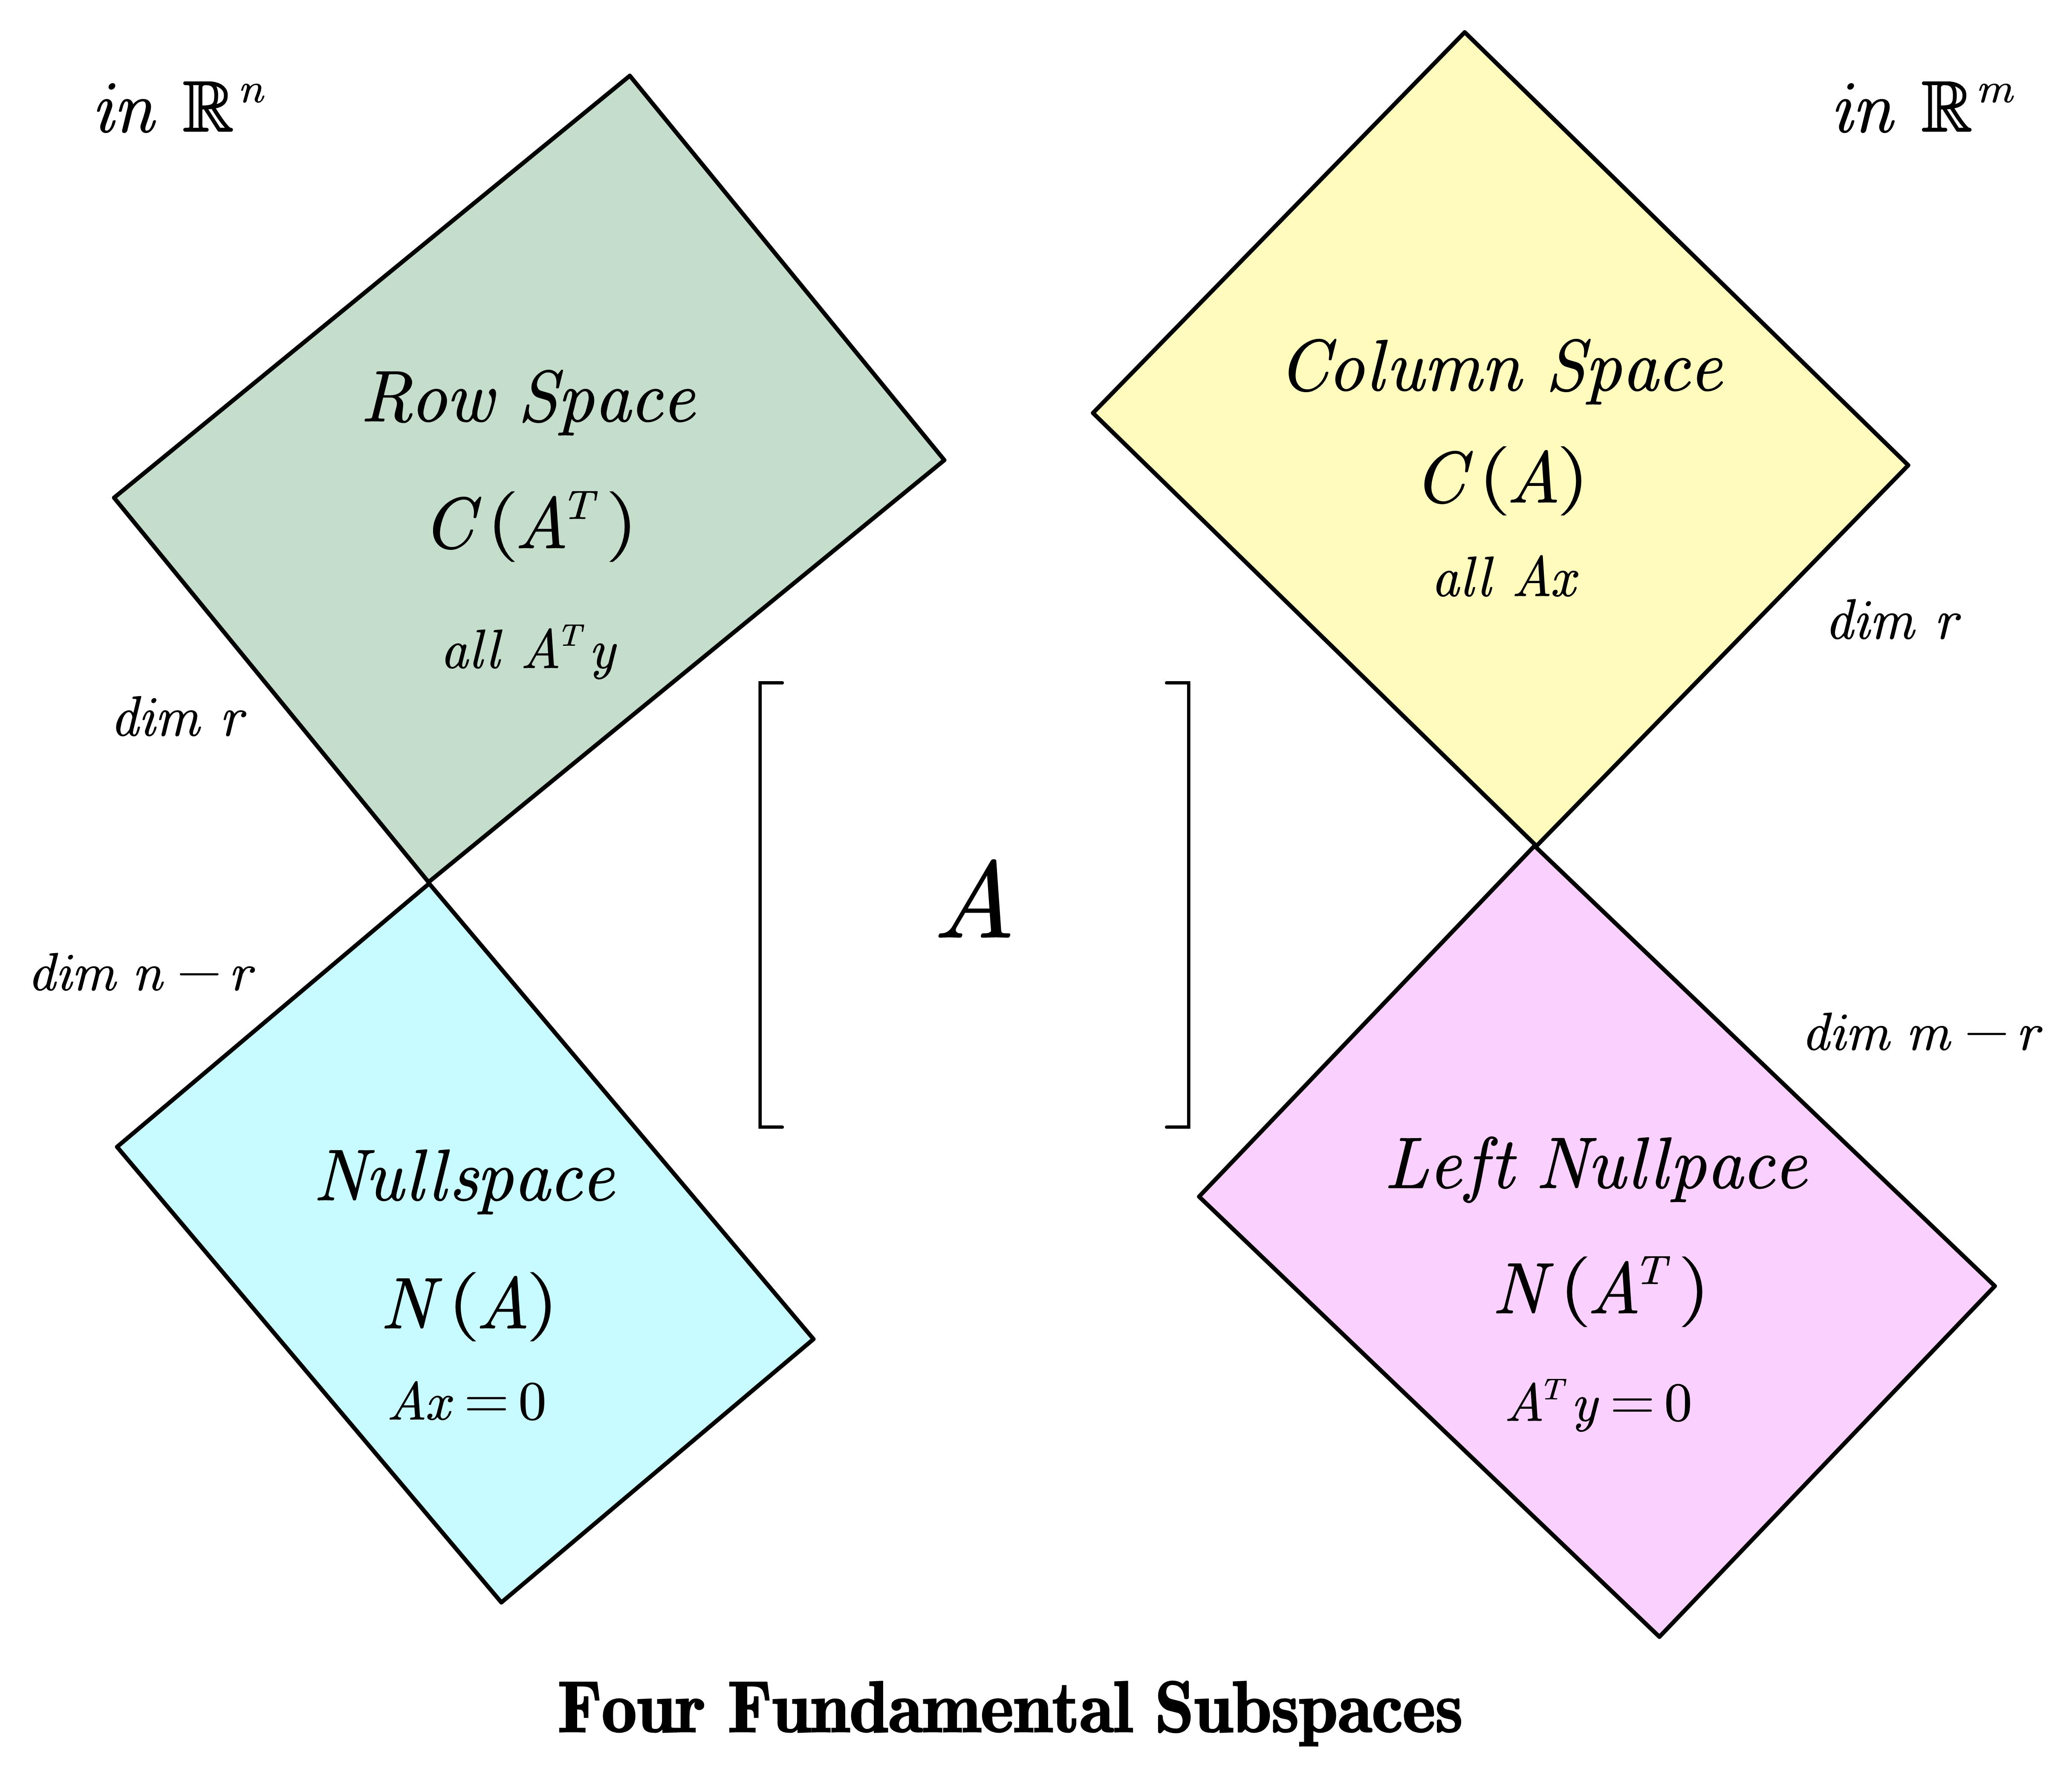
\includegraphics[width=0.74\textwidth]{subspace.jpg}
\end{center}
\end{frame}
\end{document}